\documentclass[12pt]{report}
\title{Mid Term Project}
\usepackage{amsmath}
%\usepackage{maplestd2e}
\usepackage{tikz}
\usetikzlibrary{arrows.meta,shapes.misc,patterns,shapes.symbols,decorations.pathreplacing,decorations}
\usepackage{amssymb}
\AtBeginDocument{\renewcommand{\chaptername}{}}
\usepackage{microtype}
\usepackage[bottom=30 mm, top=25 mm, left=25 mm, right=25 mm]{geometry}
\usepackage{multicol}
\usepackage{titlesec} 
\usepackage{graphicx}
\usepackage{listings}
\usepackage{xcolor}
\usepackage{subfigure}
\usepackage{subfig}
\usepackage{wrapfig}
\usepackage{float}
\usepackage{lipsum} 
\lstset{
    breaklines=true,
    tabsize=3,
    showstringspaces=false
}

\lstdefinestyle{Common}
{
    extendedchars=\true,
    language={[Visual]Basic},
    frame=single,
    framesep=3pt,
    framerule=0.4pt,
    xleftmargin=3.4pt,
    xrightmargin=3.4pt,
    rulecolor=\color{red}
}

\lstdefinestyle{A}
{
    style=Common,
    backgroundcolor=\color{yellow!10},
    basicstyle=\scriptsize\color{black}\ttfamily,
    keywordstyle=\color{orange},
    identifierstyle=\color{black},
    stringstyle=\color{red},
    commentstyle=\color{green}
}

\makeatletter 
\renewcommand\chapter{\thispagestyle{plain}%
\global\@topnum\z@
\@afterindentfalse
\secdef\@chapter\@schapter}
\makeatother 

\titleformat{\chapter}{\bfseries\Huge}{\thechapter.\quad}{0em}{}


\usepackage[utf8]{inputenc}
\parindent0pt

\begin{document}

%\setlength{\parindent}{3ex} 

\begin{large}

\thispagestyle{empty}
\begin{center}
\begin{figure}[t]
\centering

\includegraphics[scale=0.52]{sdsu_logo.png}
\end{figure}
\end{center}
\begin{center}
\Large{Department of Mathematics and Statistics}
\end{center}
\begin{center}
\Large{Prof. Joseph Mahaffy}
\end{center}
\begin{center}
\Large{Math 636, Mathematical Modeling}
\end{center}
\begin{verbatim}



\end{verbatim}
\begin{center}
\textbf{\Huge{Homework Assignment}}
\end{center}
\begin{verbatim}


\end{verbatim}
\rule{16,5 cm}{0.4pt}\\
\begin{center}
\textbf{\LARGE{Diabetes}}\\[0,7 cm]
\end{center}
\rule{16,5 cm}{0.4pt}
\begin{verbatim}


\end{verbatim}

\begin{center}
 \textbf{by Matteo Polimeno} \\ 
\textbf{11/14/2017}\\

\end{center}
\end{large}


\newpage

\tableofcontents
\newpage

\sloppy

\newpage


\chapter{Problem 1}
\section{Part c}
The model is based upon the study of Ackerman et al. on glucose-insulin regulation, a system of differential equations given by
$$
\frac{d^{2}g}{dt^{2}} + 2\alpha\frac{dg}{dt} + \omega_{0}^{2} = F(t),
$$

whose general solution is
$$
G(t) = G_{0} + Ae^{-\alpha t}cos(\omega(t-\delta)),
$$
where we have five unknown parameters to fit the data:\\

$G_{0}$ represents the equilibrium blood sugar level\\
$\alpha$ measures the ability of system to return to the equilibrium state after being perturbed\\
$\omega$ gives a frequency response to perturbations\\
$A$ gives the amplitude of the response\\
$\delta$ represents a delay in the response.\\

One of the inherent weaknesses of the model is given by the parameter $\alpha$, which was found to give many large errors in the subjects tested by Ackerman et al.; on the other hand, a strength of the model is its resemblance with the damped harmonic oscillator, which is a known system readily analyzed.\\ 
Therefore, we can use a stronger indicator of diabetes given by the natural frequency defined as
$$
\omega_{0} = \omega^{2} + \alpha^{2},
$$
which is used to compute the natural period of the system, given by
$$
T_{0}= \frac{2\pi}{\omega_{0}}.
$$
In this context, this period represents the moment in time at which most of the excess of the glucose ingested has been metabolised and the system has gone back its homeostatic conditions. We know from literature that\\

if $T_{0} < 4 \rightarrow$ Non-diabetic subject;\\
if $T_{0} > 4 \rightarrow$ Diabetic subject.\\

After running a best fit to the data given, we found that for the two subjects we have two different natural frequencies of respectively:\\

First Subject = $G_{1} \longrightarrow \omega_{0} \approx 1.903 hrs^{-1}$\\
Second Subject = $G_{2} \longrightarrow \omega_{0} \approx 1.279 hrs^{-1}$,\\

which give the following natural periods:\\

$G_{1} \longrightarrow T_{0} \approx 3.30 hrs < 4 \rightarrow$ Non-diabetic \\
$G_{2} \longrightarrow T_{0} \approx 4.9 hrs > 4 \rightarrow$ Diabetic.\\

So we found a difference of about 33\% between the two natural frequencies as well as between the two natural periods. And the situation can be visualised properly by graphing the two models along with the data given.

\begin{figure}[H]
	\centering
	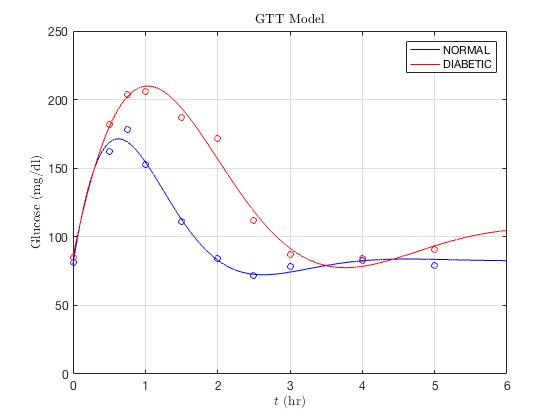
\includegraphics[scale=0.6]{DIABETES_Prob1.jpg}
	\caption{Alckerman model data-fitting}
\end{figure}

From the graph in Fig.1.1 we can see that the model fits the data really well, especially for the non-diabetic case (blu line in the graph). In fact, its Sum of Square Errors was found to be
$$
SSE_{Non-diabetic} \approx 165.7,
$$ 
whereas for the diabetic case we see some incongruences between the model and data, as it is confirmed by its SSE, found to be
$$
SSE_{Diabetic} \approx 406.33.
$$
For the non-diabetic case, we see a steady increase in the glucose level in the blood from its starting point of $G(0) = 81 mg/dL$ to its maximum found at $t \approx 0.7hrs$, so around 42 minutes after the ingestion of a large amount of glucose, to be around $G_{max}=170mg/dL$. Looking at the graph, we see that the model actually underestimates the maximum given by the data found at $t=0.75$ to be $G_{max}=178mg/dL$. Then the model fits the data almost perfectly and seems to level off after 4 hours, and at $t=4hrs$ the data from the non-diabetic subject and the diabetic subject overlap.\\
As for the diabetic case (red line in the figure), the graph fits the data reasonably well, even though it seems to be less accurate than the non-diabetic case (but it still seems to be within the margin of error). The model overestimates the maximum concentration of glucose in the blood, accurately found at $t=1hr$, therefore one hour after the ingestion of glucose, but it appears to be a value slightly greater than the $206mg/mL$ given from the data. According to the model, the level of glucose in the blood steadily increases to its maximum and then decreases to its minimum at around $t=3.7hrs$, or 3 hours and 42 minutes after the ingestion of glucose, and then increases again and appears to level off after six hours, but at a value much higher (over 100mg of glucose per dL of blood) than pre-fasting conditions.\\
The two models intersect at $t \approx 3.50$ and $t \approx 4.43$, i.e. approximately after three hours and thirty minutes and after four hours and twenty-six minutes from the ingestion of glucose. At those points the concentration of glucose in the blood is, respectively, 79mg/dL and 83.7mg/dL, and it's obviously the same for both subjects. At $t \approx 3.50$, according to the model, the non-diabetic subject sees a slight increase in the glucose level in the blood, which indeed happens according to the data given, but then it levels off after fours hours, going back to homeostatic conditions.\\
Whereas, for the diabetic subject, the model steadily decreases before the intersection point at $t \approx 3.50$, then it appears to have an interflection point immediately after and starts to steadily increase. They intersect again at $t \approx 4.43$, but, while the glucose level for the non-diabetic subject levels off, the diabetic subject sees a steady increase in the glucose concentration in the blood up until six hours after fasting, according to the model.
\\
According to a famous diabetologist, the blood glucose concentration of a non-diabetic who has just absorbed a large amount of glucose will be at or below fasting level in 2 hours or less. Using this criteria to analyse our model, we see that in fact the non-diabetic subject has a concentration of glucose in the blood of 81mg/dL before fasting; after two hours the glucose level in his/her blood is 84mg/dL, which is very close to the pre-fasting value. The level continues to drop for more than one hour after that (it's 78mg/dL at $t=3hrs$) and then increases back to 83mg/dL at $t=4hrs$. Then it decreases again, it's 79mg/dL at $t=5hrs$, and according to our model it levels off after that, indicating that all the glucose should have been absorbed.\\
For the diabetic subject we have a very different situation. Even though the two subjects start with a pretty similar pre-fasting level of glucose, 81 mg/dL for the non-diabetic case and 85mg/dL for the diabetic case, which is a difference of less than 5\%, after two hours the diabetic subject has a level of glucose in his/her blood of 172mg/dL, against the 84mg/dL of the non-diabetic case, a difference of almost 52\% between the two cases.\\
In fact, in order to go back to his/her pre-fasting level of glucose, the diabetic subject has to wait more than three hours (at $t=3hrs$ his/her level is at 87mg/dL), as we see that at $t=4hrs$ the glucose concentration is 84mg/dL. However, after that point, the glucose level seems to be increasing again as it is found to be 91mg/dL after five hours and, according to our model, seems to increase even after that point, which indicates that some therapy has to be performed on the subject in order to regulate his/her level of glucose in the blood from keeping to increase steadily.\\
Using the Oral Glucose Tolerance Test (OGTT) to analyse our data, we see that the fasting level of both subjects are below 100mg/dL and therefore, according to this standard test, both subject would be considered non-diabetic at $t=0$.\\
However, as we continue our analysis, we see that at $t=1$ the situation is quite different. In fact, the first subject has a glucose level in his/her blood of 153mg/dL, which is considered normal as it is below 180mg/dL, whereas the second subject has a glucose level in his/her blood of 206mg/dL, which is considered diabetic.\\
At $t=2$ the test suggests that non-diabetic individuals have glucose level below 140mg/dL, whereas diabetic individuals have glucose level above 180mg/dL. For our case, the first subject has glucose level of 84mg/dL after two hours from fasting, which indicates non-diabetic conditions according to the OGTT. Yet, the second subject has glucose level of 172mg/dL at $t=2$, which is way above normal conditions, but still below the value of 200mg/dL, which is considered diabetic.\\
Thus, the OGTT does not seem to be a good way for testing diabetes, as it is found to be erroneous for both  $t=0$ and $t=2$, whereas the Alkerman model represents a very good fit for the data and seems to be a better way to test diabetic conditions in individuals.

\chapter{Problem 2}
\section{Part b}
Studying the reduced 3-D model for diabetes in NOD mice by Mahaffy and Edelstein-Keshet 

$$\frac{dA}{dt} = (\sigma + \alpha_{1}M)f_{1}(p) - (\beta + \delta_{A})A - \epsilon A^{2}$$, \\
$$\frac{dM}{dt} = \beta 2^{m1}f_{2}(p)A - f_{1}(p)\alpha_{2}M - \delta_{M}M,$$\\
$$
\frac{dE}{dt}= \beta 2^{m2}(1-f_{2}(p))A - \delta_{E}E, \\
$$
$$
p \approx (RB/\delta_{p})E, \\
$$
$$f_{1}(p) = \frac{p^{n}}{k_{1}^{n} + p^{n}},$$
$$
f_{2}(p)= \frac{ak_{2}^{m}}{k_{2}^{m} + p^{m}}. \\
$$

With the parameters given in the problem, we found three equilibria.\\
The first equilibrium corresponds to the healthy state (disease-free equilibrium) and it's found to be at the origin. Thus we have
$$
(A_{e},M_{e},E_{e})= (0,0,0),
$$
where\\
A=Activated T-cells,\\ M=Memory cells,\\ E=Effector or killer T-cells.
To investigate the stability of this equilibrium we find its eigenvalues, which are found to be\\
$\lambda_{1}=-1, \lambda_{2}=-0.3, \lambda_{3}=-0.01$.\\
These values are in accordance with what was expected from literature, since we know that the characteristic equation for the Jacobian evaluated at the origin has purely negative eigenvalues given by\\
$\lambda_{1}=-\beta - \delta_{A}, \lambda_{2}=-\delta_{M}, \lambda_{3}=-\delta_{E}.$\\
Since all of the eigenvalues are real and negative, then we can conclude that the disease-free equilibrium is a stable node. Since the origin is an attractor then, for any sufficiently weak perturbation, the system should stay in this stable state, meaning that if a disturbance takes place altering the homeostatic conditions of the mice, the situation will tend to stabilyse. Biologically speaking, in this case there are no activated T-cells, therefore they cannot kill $\beta$-cells and Type-1 diabetes will not rise, so the mice stay healthy.\\

The second equilibrium is found at 
$$
(A_{e},M_{e},E_{e})= (0.1255,0.0141,0.0374).
$$
This is the diseased-state equilibrium and the eigenvalues are found to be\\
$\lambda_{1}=-2.4183, \lambda_{2,3}=0.0089 \pm 0.5702i$.\\
So in this case we have one real eigenvalue and a pair of complex conjugates, whose real part has opposite sign to the real eigenvalue. This indicates that the diseased equilibrium is a so-called saddle-focus: it has an attractive direction in one dimension (an attractive line) connected to the real eigenvalue and a repulsive direction in two dimensions connected to the complex eigenvalues (a repelling spiral plane). This type of equilibrium is always unstable, so we can say that the diseased-state equilibrium is an unstable node.\\
Biologically, this equilibrium corresponds to a state of elevated immune-cells level. Basically, T-cells have been activated (in fact $A$ is greater than zero) and many of them have become Effector T-cells (cytotoxic T-lymphocytes or CTLs). CTLs are efficient specific killers which continuously attack and destroy $\beta$-cells in the pancreas. This is an autoimmune attack that leads to diabetes. Since this equilibrium is unstable, then only the origin is an attractor.\\

The third equilibrium is found at
$$
(A_{e},M_{e},E_{e})= (0.0162,1.1294,0.00108).
$$
We know from literature that this is a saddle node and its eigenvalues confirm that, as they are found to be\\
$\lambda_{1}=-1.534, \lambda_{2}=-0.0188, \lambda_{3}=0.2095$.\\
Since we have two negative eigenvalues (which indicate an attractive direction) and one positive eigenvalue (repelling direction), this equilibrium is in fact a saddle node. Therefore, it has a 2-D stable manifold (a plane that is locally attracted to the saddle node) and a 1-D unstable manifold (a line that is locally repelled away from the saddle node).\\
In order to better investigate its behavior, we simulate this system with a different set of initial conditions and we plot the results:

\begin{figure}[H]
	\subfigure[]{\includegraphics[scale=0.6]{Quasi_Steady_Part1.jpg}}
	\subfigure[]{\includegraphics[scale=0.6]{Quasi_Steady_Part1_Zoom3.jpg}}
	\caption{a)QSS Model - Simulation; b) Zoom in on stable oscillations}
\end{figure}

We see from Fig.2.1a that when there are no Activated T-cells ($A$ value) and consequently no Effector T-cells ($E$ value), then for any nonzero value of the memory cells ($M$ value), all solutions will tend towards the healthy state located at the origin, as it can be seen by looking at the red line in Fig.2.1a.\\
On the other hand, when $A> 0$, we see that the solutions tend to oscillate in a stable manner around the diseased-state, as can be readily seen by zooming in on the plot (Fig.2.1b).\\ So, globally, if there is a nonzero number of T-cells that have been activated, which seems to be a reasonable outcome for many T-cells that undergo a set of interactions with antigen presenting cells (APCs) in the Lymph nodes, then the system will tend to oscillate around the diseased-state. Thus, T-cells will continuously kill $\beta$-cells, generating an autoimmune attack that will lead to the mice getting diabetes. This is also confirmed by looking at the given value of the peptide clearance rate $\delta_{p}=1$, a parameter that is often studied, as it is believed that poor clearance could induce diabetes. The normal range for $\delta_{p}$ is considered to be between 2.5 and 3.5. In our case, we have a value of 1 which is less than half the normal range of values for $\delta_{p}$ and this corresponds to a diseased-state. Since we do not have a normal state, then we can say something more about the nature of the manifolds found for the third equilibrium: for our given values of the parameters, the 2-D stable manifold separates the healthy-state from the diseased equilibria. Since we see that most solutions oscillate around the saddle node, then it is reasonable to say that most stimuli fall on the wrong side of the separatrix and are attracted to the diseased-equilibrium.\\
In conclusion, it is reasonable to state that the mice will get diabetes in this case of study.\\

\section{Part c}

In this case of study the value of the parameter $\delta_{p}$ has been changed from 1 to 1.5.\\
The first equilibrium corresponds to the healthy state (disease-free equilibrium) and it's again found to be at the origin. Thus we have
$$
(A_{e},M_{e},E_{e})= (0,0,0).
$$

To investigate the stability of this equilibrium we find its eigenvalues, which are found to be\\
$\lambda_{1}=-1, \lambda_{2}=-0.3, \lambda_{3}=-0.01$,\\
which correspond to the same values found in the previous case, as expected since the values of the constant $\beta, \delta_{A}, \delta_{M}, \delta_{E}$ are left unchanged.

Once again, since all the eigenvalues are real and negative, we can conclude that the disease-free equilibrium is a stable node. Since the origin is an attractor, then, for any sufficiently weak perturbation, the system should stay in this stable state, meaning that if a disturbance takes place altering the homeostatic conditions of the mice, the system will tend back towards stability. Biologically speaking, in this case there are no activated T-cells, therefore there are no effector T-cells to kill $\beta$-cells and Type-1 diabetes cannot rise, so the mice stay healthy.\\

The second equilibrium is found at 
$$
(A_{e},M_{e},E_{e})= (0.1844,0.0231,0.0544).
$$
This is the diseased-state equilibrium and the eigenvalues are found to be\\
$\lambda_{1}=-2.5013, \lambda_{2,3}=0.0099 \pm 0.5735i$.\\
So in this case we have one real eigenvalue and a pair of complex conjugates, whose real part has opposite sign to the real eigenvalue. This indicates that the diseased equilibrium is a so-called saddle-focus: it has an attractive direction in one dimension (an attractive line) connected to the real eigenvalue and a repulsive direction in two dimensions connected to the complex eigenvalues (a repelling spiral plane). This type of equilibrium is always unstable, so we can say that the diseased-state equilibrium is an unstable node.\\
Biologically, this equilibrium corresponds to a state of elevated immune-cells level. Basically, T-cells have been activated (in fact $A$ is greater than zero) and many of them have become Effector T-cells (cytotoxic T-lymphocytes or CTLs). CTLs are efficient specific killers which continuously attack and destroy $\beta$-cells in the pancreas. This is an autoimmune attack that leads to diabetes. Since this equilibrium is unstable, then only the origin is an attractor.\\

The third equilibrium is found at
$$
(A_{e},M_{e},E_{e})= (0.0244,1.7001,0.0016).
$$
We know from literature that this is a saddle node and its eigenvalues confirm that, as they are found to be\\
$\lambda_{1}=-1.549, \lambda_{2}=-0.0188, \lambda_{3}=0.2077$.\\
Since we have two negative eigenvalues (which indicate an attractive direction) and one positive eigenvalue (repelling direction), this equilibrium is in fact a saddle node. Therefore, it has a 2-D stable manifold (a plane that is locally attracted to the saddle node) and a 1-D unstable manifold (a line that is locally repelled away from the saddle node).\\
In order to better investigate its behavior, we simulate this system with a different set of initial conditions and we plot the results:

\begin{figure}[H]
	\subfigure[]{\includegraphics[scale=0.6]{Quasi_Steady_Part2.jpg}}
	\subfigure[]{\includegraphics[scale=0.6]{Quasi_Steady_Part2_Zoom.jpg}}
	\caption{a)QSS Model - Simulation; b) Zoom in on stable oscillations}
\end{figure}

We see from Fig.2.2a that when there are no Activated T-cells ($A$ value) and consequently no Effector T-cells ($E$ value), then for any nonzero value of the memory cells ($M$ value), all solutions will tend towards the healthy state located at the origin, as it can be seen by looking at the green line in Fig.2.2a.\\
On the other hand, when $A> 0$, we see that the solutions tend to oscillate in a stable manner around the diseased-state, as can be readily seen by zooming in on the plot (Fig.2.2b).\\ So, globally, if there is a nonzero number of T-cells that have been activated, which seems to be a reasonable outcome for many T-cells that undergo a set of interactions with antigen presenting cells (APCs) in the Lymph nodes, then the system will tend to oscillate around the diseased-state. Thus, T-cells will continuously kill $\beta$-cells, generating an autoimmune attack that will lead to the mice getting diabetes. This is also confirmed by looking at the given value of the peptide clearance rate $\delta_{p}=1.5$. The normal range for $\delta_{p}$ is considered to be between 2.5 and 3.5. In our case, we have a value of 1.5 which is about half the normal range of values for $\delta_{p}$. \\
Also, since we do not have a normal state, we can say that, for our given values of the parameters, the 2-D stable manifold separates the healthy-state from the diseased equilibria. Since we see that most solutions oscillate around the saddle node, then it is reasonable to say that most stimuli fall on the wrong side of the separatrix and are attracted to the diseased-equilibrium.\\

To further analyse the system we should also consider the following relationship
$$
p \approx \frac{RB}{\delta_{p}}E,
$$
which is the Quasi-Steady State peptide expression, where $B$ is the fraction of remaining $\beta$-cells and $R$, for our intended purposes, is a constant.\\
Since the value of $\delta_{p}$ has increased by 50\%, we expect the value of $p$ to decrease, as the other parameters are left untouched. Because of their inversely proportional relationship, an increase in $\delta_{p}$ is equivalent to a decrease in $B$, which means more $\beta$-cells would be dying. Therefore, compared to our previous system, in this case we should have a higher number of dying $\beta$-cells, which implies a higher number of activated T-cells and hence a higher number of effector T-cells. So the $\beta$-cells of the mice are likely killed at a higher rate than in the previous case, hence diabetic conditions should rise faster.\\
However, locally the situation appears rather similar in both cases, if we just look at the graphs. In fact, as we can see in Fig.2.2b, most solutions tend to oscillate in a stable manner around the diseased-state equilibrium. The main difference appear to be an increase in the amplitude of the oscillations around the saddle node (diseased-equilibrium), as expected by the increase in the value of $\delta_{p}$.\\
Globally, the qualitative behavior is similar to the previous case of study as the mice will still get diabetes in this case, as well.



%\chapter{Problem 3}
%\input{Problem3_Latex}

%\chapter{Computational Application}
%\input{chapter4}





\end{document}
